%%%%%%%%%%%%%%%%%%%%%%%%%%%%%%%%%%%%%%%%% 
% Beamer Presentation
% LaTeX Template
% Version 1.0 (10/11/12)
% 
% This template has been downloaded from:
% http://www.LaTeXTemplates.com
% 
% License:
% CC BY-NC-SA 3.0 (http://creativecommons.org/licenses/by-nc-sa/3.0/)
% 
%%%%%%%%%%%%%%%%%%%%%%%%%%%%%%%%%%%%%%%%% 

% ----------------------------------------------------------------------------------------
%	PACKAGES AND THEMES
% ----------------------------------------------------------------------------------------

\documentclass{beamer}

\mode<presentation> {

  % The Beamer class comes with a number of default slide themes
  % which change the colors and layouts of slides. Below this is a list
  % of all the themes, uncomment each in turn to see what they look like.

  % \usetheme{default}
  % \usetheme{AnnArbor}
  % \usetheme{Antibes}
  % \usetheme{Bergen}
  % \usetheme{Berkeley}
  % \usetheme{Berlin}
  % \usetheme{Boadilla}
  % \usetheme{CambridgeUS}
  % \usetheme{Copenhagen}
  % \usetheme{Darmstadt}
  % \usetheme{Dresden}
  % \usetheme{Frankfurt}
   \usetheme{Goettingen}
  % \usetheme{Hannover}
  % \usetheme{Ilmenau}
  % \usetheme{JuanLesPins}
  % \usetheme{Luebeck}
  % \usetheme{Madrid}
  % \usetheme{Malmoe}
  % \usetheme{Marburg}
  % \usetheme{Montpellier}
  % \usetheme{PaloAlto}
  % \usetheme{Pittsburgh}
  % \usetheme{Rochester}
  % \usetheme{Singapore}
  % \usetheme{Szeged}
  % \usetheme{Warsaw}

  % As well as themes, the Beamer class has a number of color themes
  % for any slide theme. Uncomment each of these in turn to see how it
  % changes the colors of your current slide theme.

  % \usecolortheme{albatross}
  % \usecolortheme{beaver}
  % \usecolortheme{beetle}
  % \usecolortheme{crane}
  % \usecolortheme{dolphin}
  % \usecolortheme{dove}
  % \usecolortheme{fly}
  % \usecolortheme{lily}
  % \usecolortheme{orchid}
  % \usecolortheme{rose}
  % \usecolortheme{seagull}
  % \usecolortheme{seahorse}
  % \usecolortheme{whale}
  % \usecolortheme{wolverine}

  % \setbeamertemplate{footline} % To remove the footer line in all slides uncomment this line
   \setbeamertemplate{footline}[page number] % To replace the footer line in all slides with a simple slide count uncomment this line

  % \setbeamertemplate{navigation symbols}{} % To remove the navigation symbols from the bottom of all slides uncomment this line
}

\usepackage{graphicx} % Allows including images
\usepackage{booktabs} % Allows the use of \toprule, \midrule and \bottomrule in tables
\usepackage[german]{babel} % Required to compile in Windows
\usepackage[latin1]{inputenc}
\usepackage{caption}
\usepackage{subcaption}
%\usepackage{physics}
\usepackage{mathtools}
\usepackage{natbib}
\usepackage[T1]{fontenc}


\AtBeginSection[]{
  \begin{frame}
    \vfill
    \centering
    \begin{beamercolorbox}[sep = 8pt, center, shadow = true, rounded = true]{title}
      \usebeamerfont{title}\insertsectionhead\par%
    \end{beamercolorbox}
    \vfill
  \end{frame}
}

% ----------------------------------------------------------------------------------------
%	TITLE PAGE
% ----------------------------------------------------------------------------------------

\title[Hochselektive Oktavfilterbank]{Hochselektive Oktavfilterbank}

\author[]{Erik Engelhardt, Jan Heimann, Oliver Kochan, Christopher Rotzlawski} % Your name
\institute[HAW] % Your institution as it will appear on the bottom of every slide, may be shorthand to save space
{
  FH Westk�ste \\ % Your institution for the title page

  \medskip
%  \textit{erik.engelhardt@haw-hamburg.de} % Your email address
}
\date{\today} % Date, can be changed to a custom date

\begin{document}

\begin{frame}
  \titlepage % Print the title page as the first slide
\end{frame}

\begin{frame}[allowframebreaks]
  %\frametitle{Gliederung} % Table of contents slide, comment this block out to remove it
  \tableofcontents % Throughout your presentation, if you choose to use \section{} and \subsection{} commands, these will automatically be printed on this slide as an overview of your presentation
\end{frame}

% ----------------------------------------------------------------------------------------
%	PRESENTATION SLIDES
% ----------------------------------------------------------------------------------------

\section{Einleitung}

\begin{frame}
\frametitle{Hochselektive Filterbank in Br�ckenstruktur}
\begin{itemize}
	\item Oktav-Filterbank mit bis zu 9 Teilb�ndern
	\item Bieziproke Teilbandfilter
	\item Simulation mit Python
	\item Hardwarerealisation auf DSP TMS320C6713
\end{itemize}
\end{frame}

\section{Grundlagen}

\begin{frame}
\frametitle{Bireziproker Teilbandfilter}
\end{frame}

\begin{frame}
\frametitle{Oktav-Filterbank}
\end{frame}

\section{Simulation}

\subsection{Umgebung}

\begin{frame}
  \frametitle{Simulationsumgebung}
  \begin{itemize}
  \item Simulation der Filterbank in Python
    \begin{itemize}
    \item Numpy Modul der Scipy-Bibliothek~\cite{scipy} f�r Berechnungen und Datenstruckturen
    \item Matplotlib-Bibliothek zum Erstellen der Diagramme~\cite{Hunter:2007}
    \end{itemize}
  \end{itemize}
\end{frame}

\subsection{Implementierung}

\begin{frame}
  \frametitle{Klassendiagramm}
  \begin{itemize}
  \item Simulation in zwei Schritten
    \begin{itemize}
    \item update()
    \item advance()
    \end{itemize}
  \item Einstellen der Ordnung �ber Parameter T
  \end{itemize}
  \begin{figure}
    \centering
    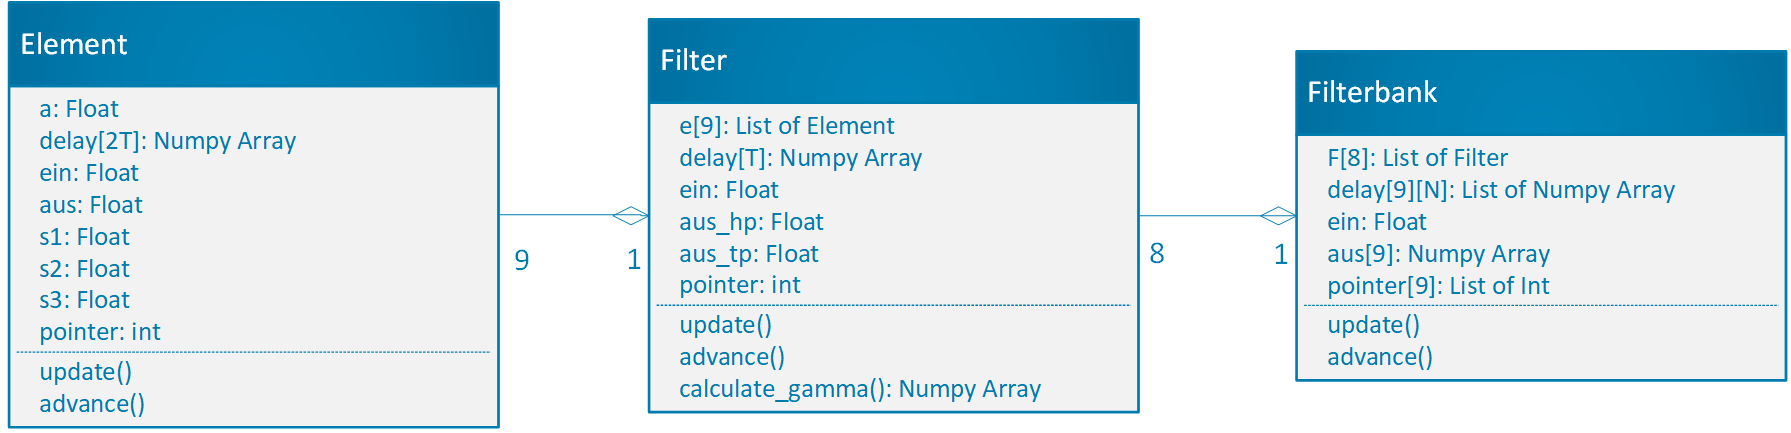
\includegraphics[width=1\textwidth]{img/klassendia}
    \caption{Klassendiagramm f�r die Implementierung einer hochselektiven Filterbank}\label{fig:impl_klassdia}
  \end{figure}
\end{frame}

% \begin{frame}
%   \frametitle{Element}
%   \begin{itemize}
%   \item Repr�sentiert einen Adaptor
%   \end{itemize}
%   \begin{figure}[h!]
%     \centering	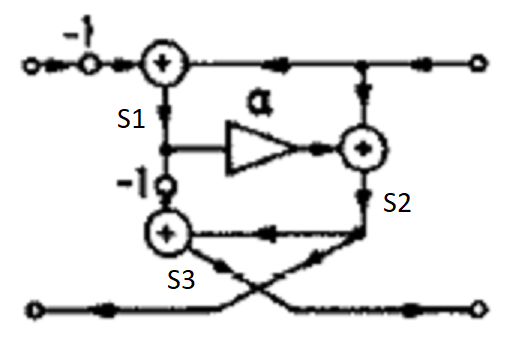
\includegraphics[width=10cm]{img/Adapter.png}
%     \caption{Verwendeter Adaptor f�r den bireziproken Wellendigitalfilter \cite[][S. 77]{gaszi1983}}\label{fig:Adaptor}
%   \end{figure}
% \end{frame}

% \begin{frame}
%   \frametitle{Filter}
%   \begin{itemize}
%   \item Besteht aus 9 \emph{Elementen} bzw. Adaptoren und einem Verz�gerungsglied
%   \end{itemize}
%   \begin{figure}[h!]
%     \centering	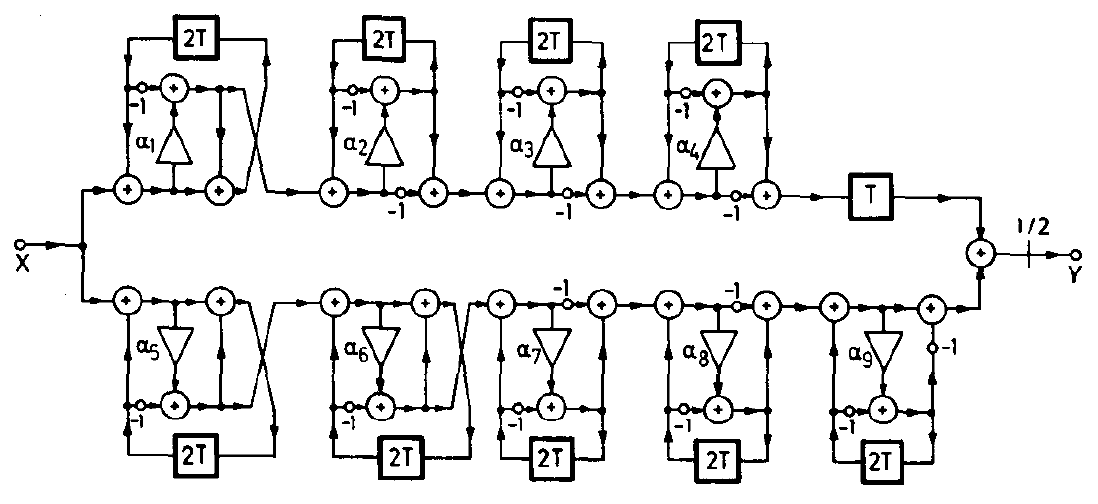
\includegraphics[width=15cm]{img/BireziprokerFilter.png}
%     \caption{Grundstruktur des bireziproken Wellendigitalfilters \cite[][S. 85]{gaszi1983}}\label{fig:bireziprok_Struktur}
%   \end{figure}
% \end{frame}

% \begin{frame}
%   \frametitle{Filterbank}
%   \begin{itemize}
%   \item Besteht aus 8 Teilfiltern und Verz�gerungsgliedern
%   \end{itemize}
%   \begin{figure}[h!]
%     \centering	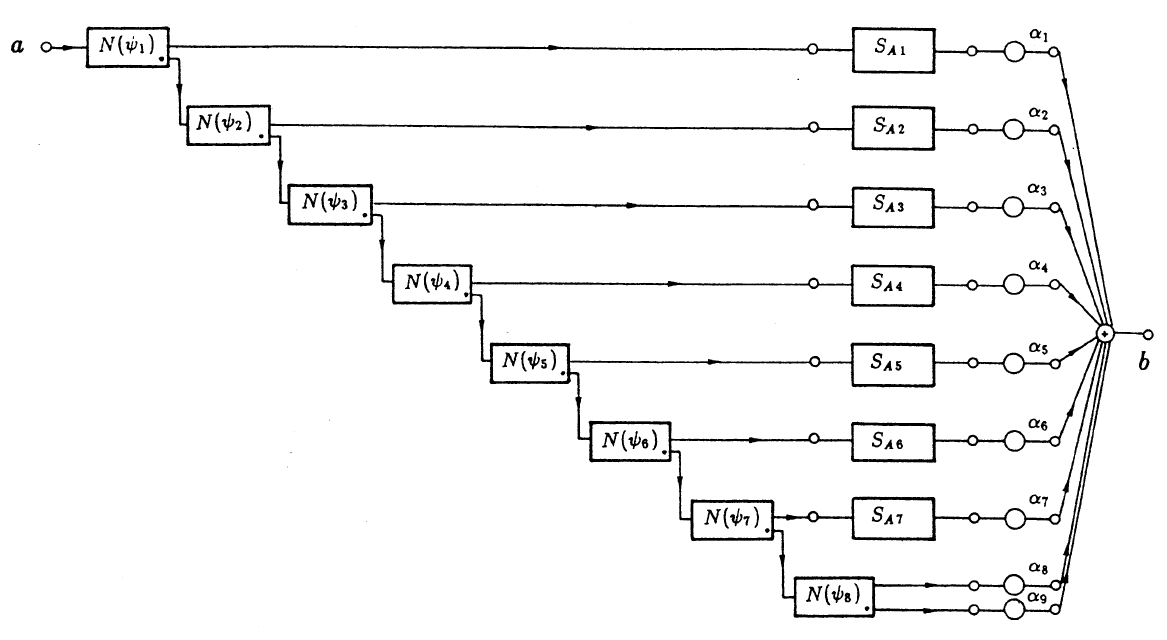
\includegraphics[width=15cm]{img/OktavFilter.png}
%     \caption{Oktav-Filterbank mit neun Teilb�ndern \cite[][S. 95]{kunold1989}}\label{fig:OktavFilterbank}
%   \end{figure}  
% \end{frame}

\subsection{Ergebnisse}

\begin{frame}
  \frametitle{Erstes Teilband im Frequenzbereich}
  \begin{figure}[h!]
    \centering	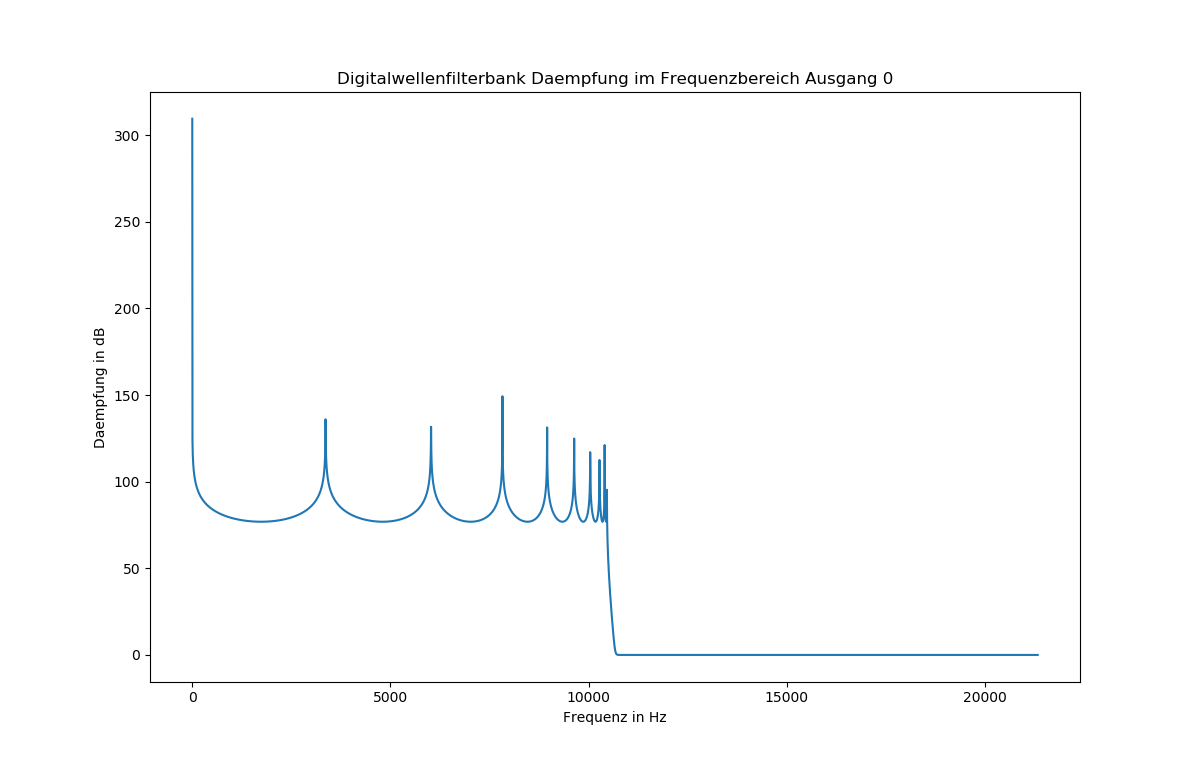
\includegraphics[width=\textwidth]{img/bank_freq_0.png}\caption{Ausgang des ersten Teilbandes}
    \label{fig:Teilband0}
  \end{figure}  
\end{frame}

\begin{frame}
  \frametitle{Sechstes Teilband im Frequenzbereich}
  \begin{figure}[h!]
    \centering	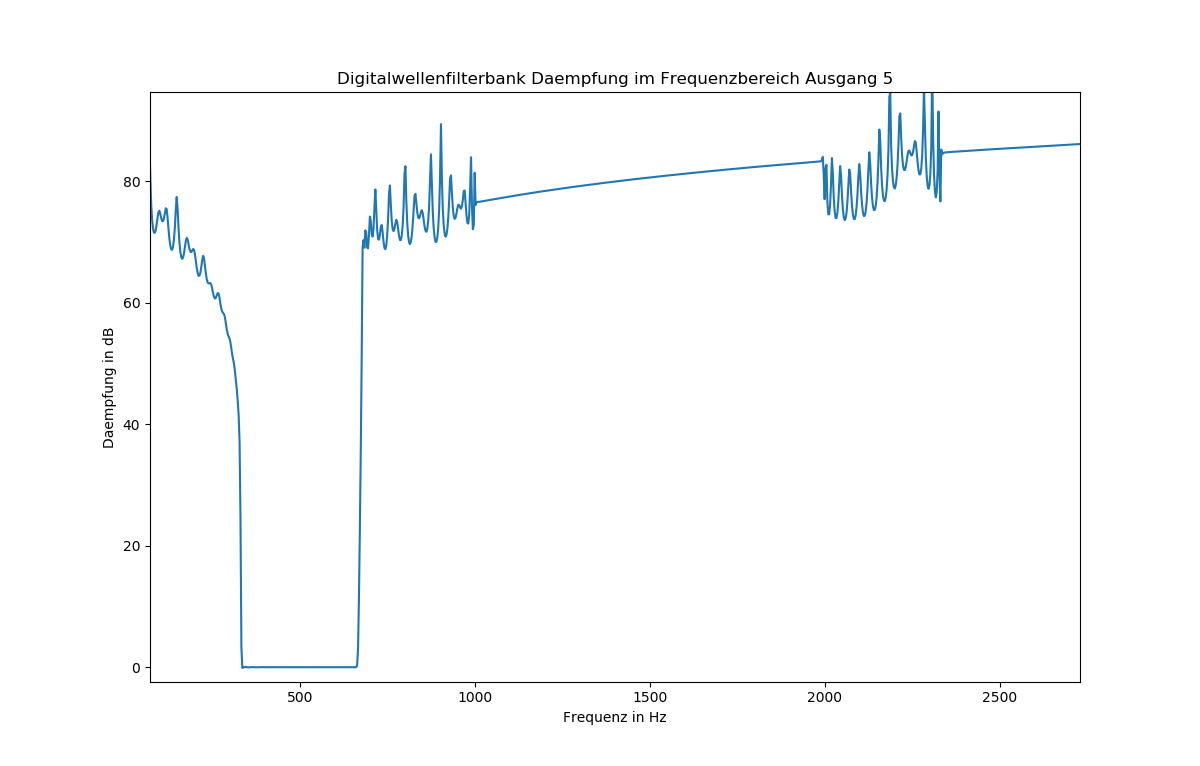
\includegraphics[width=\textwidth]{img/bank_freq_5_close.png}
  \caption{Ausgang des sechsten Teilbandes}\label{fig:Teilband5}
  \end{figure}
\end{frame}

\begin{frame}
  \frametitle{Filterbankausgang im Frequenzbereich}
  \begin{itemize}
  \item Abweichung vom optimalen Allpass-Verlauf bei den �berg�ngen zwischen den Teilb�ndern
  \end{itemize}
  \begin{figure}[h!]
    \centering	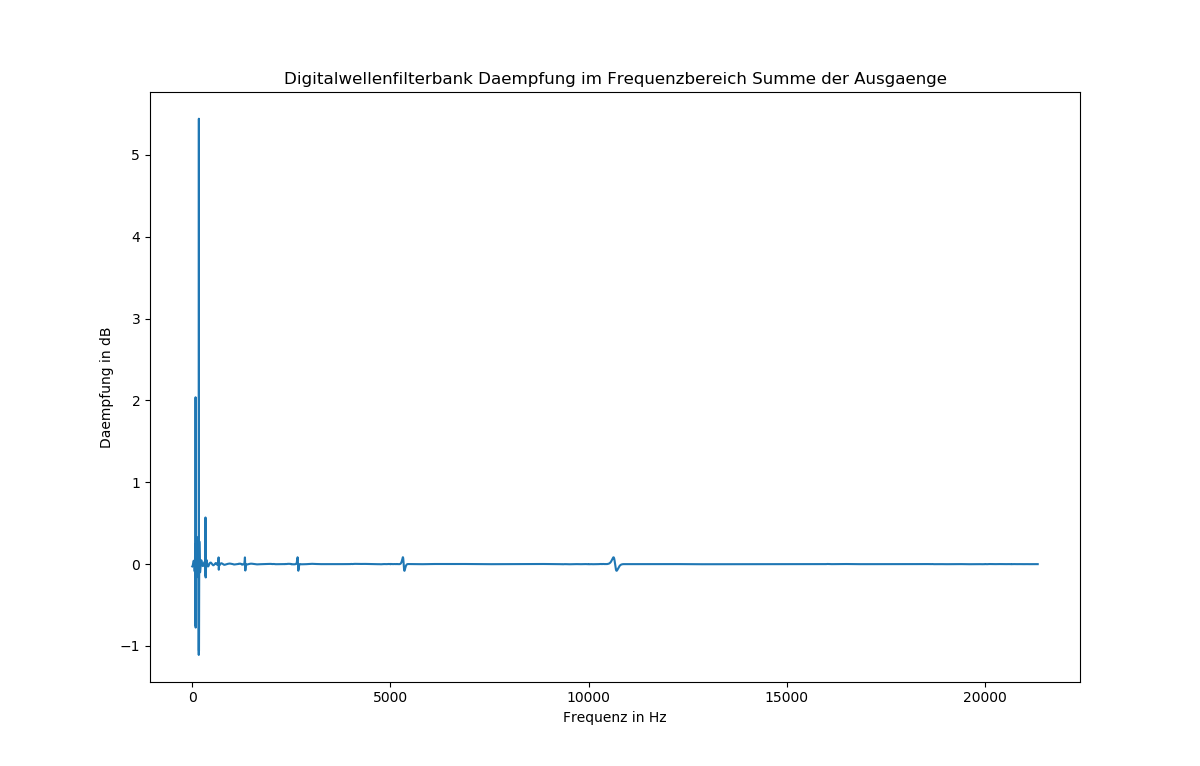
\includegraphics[width=\textwidth]{img/bank_freq_summe_keinAusgleich.png}
    \caption{D�mpfung der Oktav-Filterbank ohne Laufzeitausgleich}\label{fig:AusgangDeampfung}
\end{figure}
\end{frame}

\begin{frame}
  \frametitle{Ausgleich der Signallaufzeiten}
  \begin{itemize}
  \item Ermittlung der Signallaufzeiten durch Ablesen der Maxima der einzelnen Teilb�nder
  \item Letzes Teilband hat Maximum nach 1500 Takten
  \end{itemize}
  \begin{figure}[h!]
    \centering	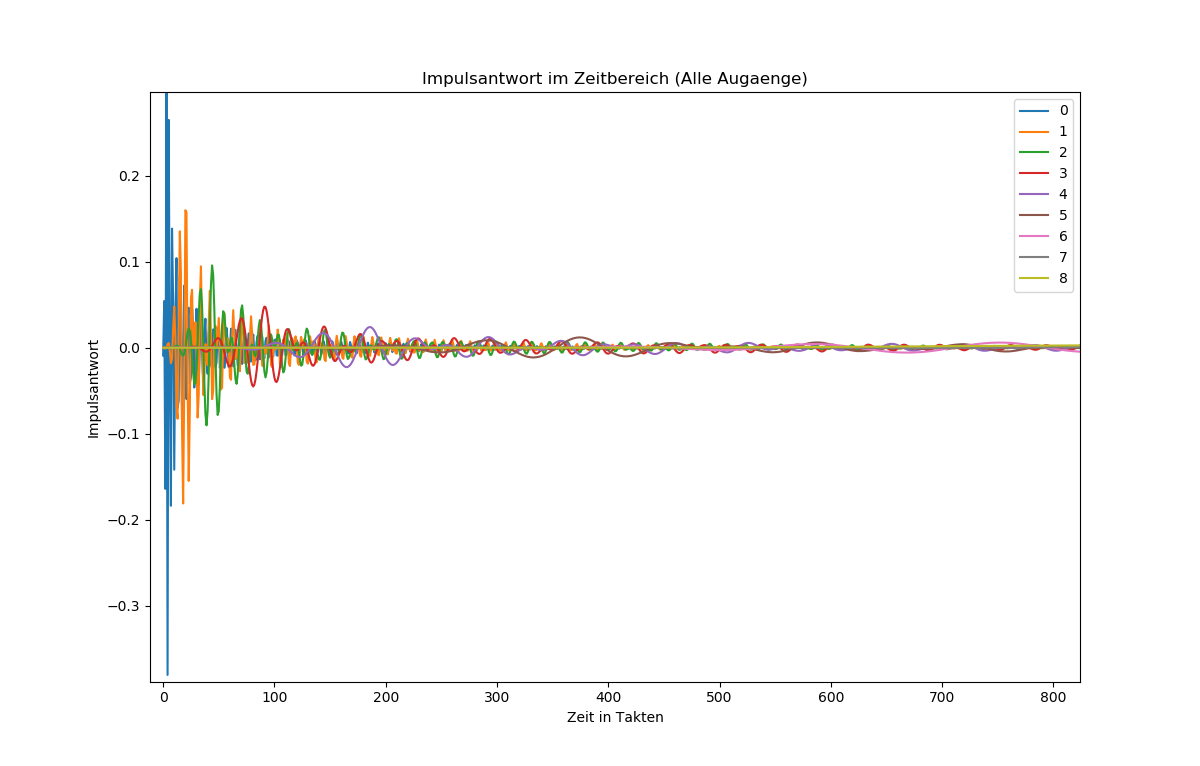
\includegraphics[width=\textwidth]{img/bank_zeit_alle_keinAusgleich.png}
    \caption{Signallaufzeiten der Teilfilterb�nder ohne Ausgleich}\label{fig:TeilbandLaufzeitenohne}
  \end{figure}
\end{frame}

\begin{frame}
  \frametitle{Ausgleich der Singallaufzeiten}
  \begin{itemize}
  \item Verz�gerung der schnelleren Ausg�nge auf Laufzeit des langsamsten Ausgangs
  \end{itemize}
  \begin{figure}[h!]
    \centering	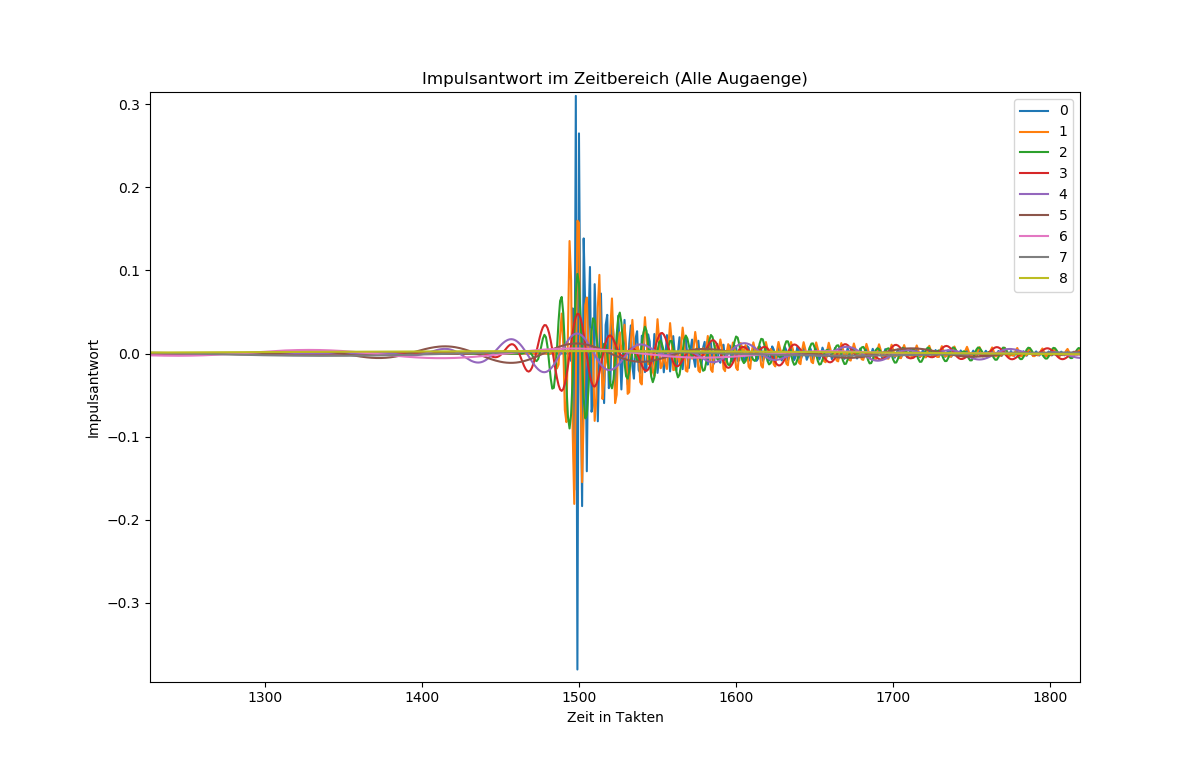
\includegraphics[width=\textwidth]{img/bank_zeit_alle.png}
    \caption{Signallaufzeiten der Teilfilterb�nder}\label{fig:TeilbandLaufzeiten}
\end{figure}

\end{frame}

\begin{frame}
  \frametitle{Filterbankausgang im Frequenzbereich}
  \begin{itemize}
  \item Geringere Abweichung vom optimalen Verlauf durch Laufzeitausgleich
  \end{itemize}
  \begin{figure}[h!]
    \centering	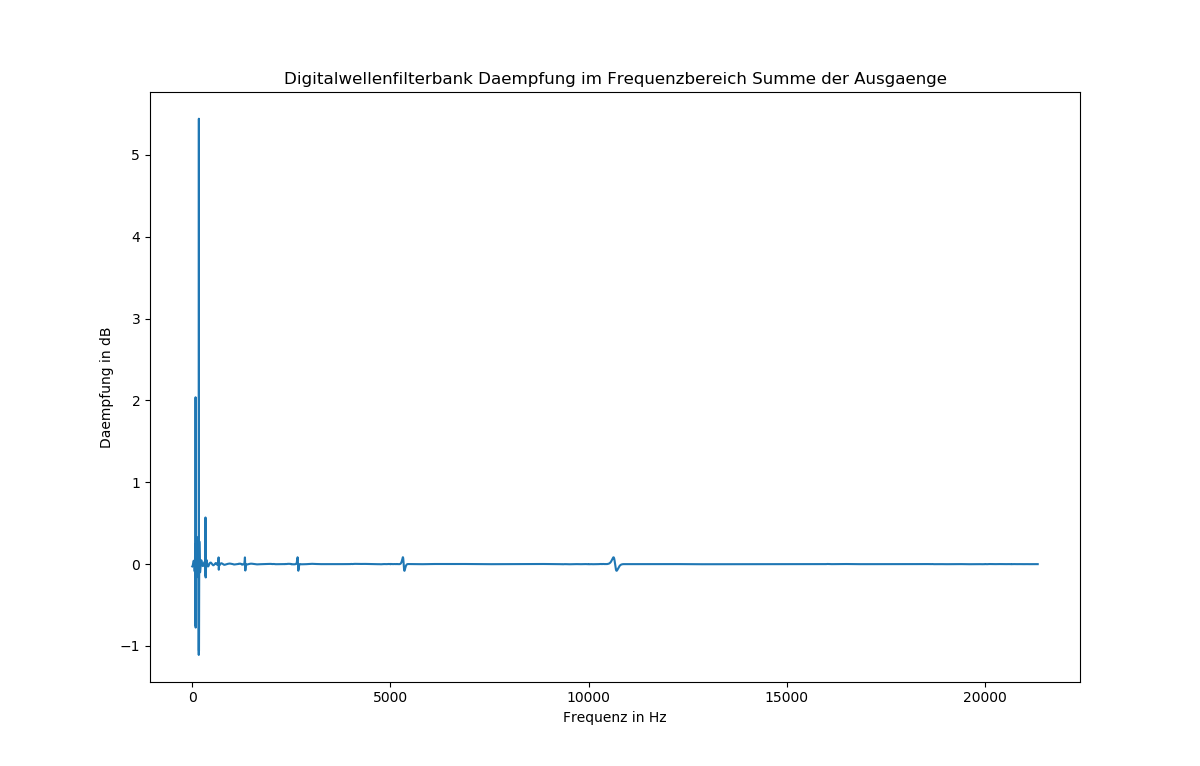
\includegraphics[width=\textwidth]{img/bank_freq_summe_keinAusgleich.png}
    \caption{D�mpfung der Oktav-Filterbank mit Laufzeitausgleich}\label{fig:AusgangDeampfung}
\end{figure}
\end{frame}

\section{Realisierung}
    \begin{frame}
        \begin{itemize}
            \item Entwicklungshardware:
            \begin{itemize}
                \item Spectrum Digital \emph{DSK6713}
                \item CPU: Texas Instruments \emph{TMS320C6713} floating-point DSP
            \end{itemize}
            \item Messequipment
            \begin{itemize}
                \item AudioTester
                \item PicoScope AWG + Oszilloskop
                \item Rohde \& Schwarz UPV Audio Analyser  
            \end{itemize}
        \end{itemize}
    \end{frame}

    \begin{frame}
        \begin{itemize}
            \item Filterstruktur der Teilbandfilter nach Gaszi
        \end{itemize}
        \begin{figure}[b]
            \centering
            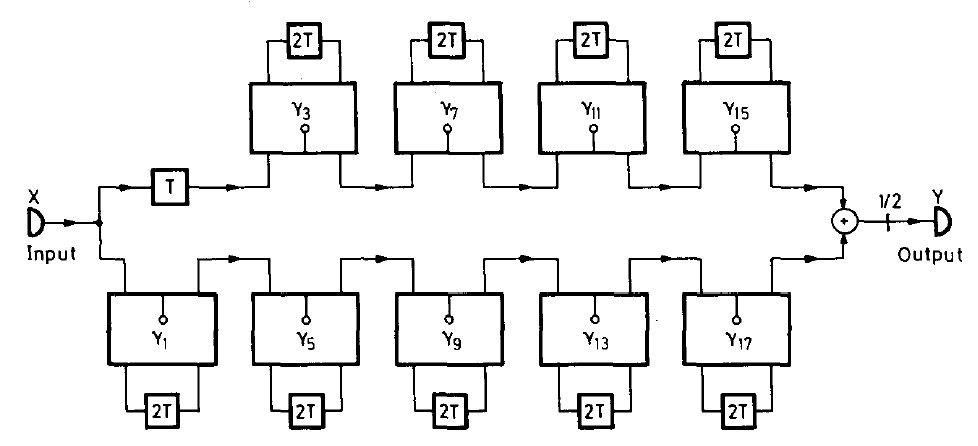
\includegraphics[width=\textwidth]{img/Teilbandfilter.png}
            \caption{Struktur eines Teilbandfilters \citep[Abb. 14a]{gaszi1983}}
        \end{figure}    
    \end{frame}

    \begin{frame}
        \begin{itemize}
            \item Flie�kommaarithmetik
            \begin{itemize}
                \item Optimierungen f�r Festkommaarithmetik in Q15 entfallen
                \item Einheitliche Struktur der Adaptore
            \end{itemize}
        \end{itemize}
        \begin{figure}[b]
            \centering
            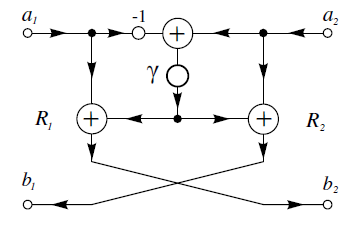
\includegraphics[width=0.7\textwidth]{img/Adaptor.png}
            \caption{Symmetrischer Zweitor-Paralleladaptor \citep{bvdsv}}
        \end{figure}
    \end{frame}

    \begin{frame}
        \begin{itemize}
            \item Einlesen und Ausgeben der Samples �ber DMA
            \begin{itemize}
                \item Maximierung der verf�gbaren Rechenzeit f�r die Filterberechnung
                \item Blockgr��e: 8 Samples ~~\dots~~ 2048 Samples
            \end{itemize}
        \end{itemize}
    \end{frame}

\subsection{Verarbeitung}
    \begin{frame}
        \begin{figure}[p]
            \centering
            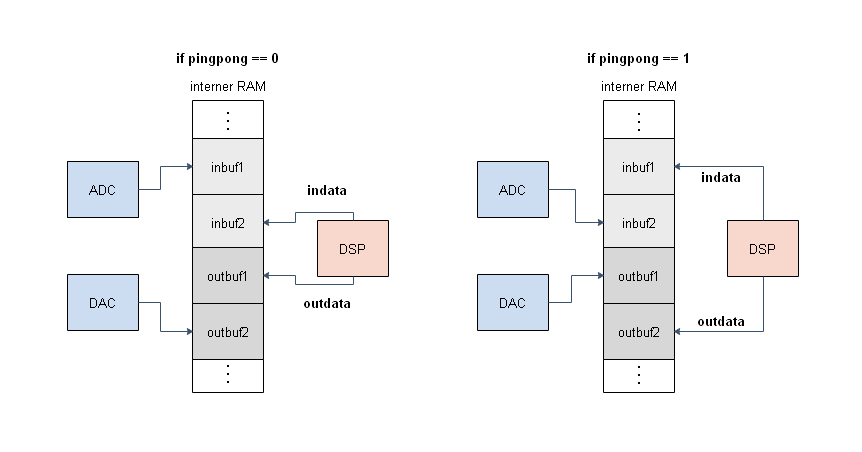
\includegraphics[width=\textwidth]{img/dma_zugriff.png}
            \caption{DMA-Pingpong}
        \end{figure}
    \end{frame}

    \begin{frame}
        \begin{figure}[p]
            \centering
            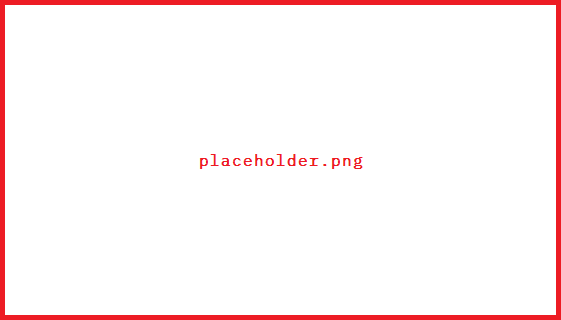
\includegraphics[width=\textwidth]{img/placeholder.png}
            \caption{Schematische Darstellung eines Ringpuffers}
        \end{figure}
    \end{frame}

\subsection{Optimierung}
    \begin{frame}
        \begin{itemize}
            \item Erster Ansatz: ohne Optimierung
            \begin{itemize}
                \item DMA Blockgr��e: 8 Samples
                \item Delaylines als lineare Puffer realisiert
                \item $\rightarrow$ 0 Teilbandfilter
            \end{itemize}
        \end{itemize}
        \begin{itemize}
            \item 1. Optimierungsschritt
            \begin{itemize}
                \item Compileroptimierung auf Stufe 1
                \item $\rightarrow$ 3 Teilbandfilter
            \end{itemize}
        \end{itemize}
        \begin{itemize}
            \item 2. Optimierungsschritt
            \begin{itemize}
                \item Delaylines f�r Adaptore als Ringpuffer realisiert
                \item $\rightarrow$ 6 Teilbandfilter
            \end{itemize}
        \end{itemize}
    \end{frame}

    \begin{frame}
        \begin{itemize}
            \item Entzerrung hinzugef�gt
            \begin{itemize}
                \item DMA Blockgr��e: 2048 Samples
                \item $\rightarrow$ 6 Teilbandfilter
            \end{itemize}
            \item Letzter Optimierungsschritt
            \begin{itemize}
                \item S�mtliche Delaylines als Ringpuffer realisiert
                \item Ersetzen der Modulo-Funktion
                \item $\rightarrow$ 7 Teilbandfilter
            \end{itemize}
        \end{itemize}
        \begin{itemize}
            \item Weitere Optimierungsma�nahmen ohne Wirkung
            \begin{itemize}
                \item Verg��erung der Ein- und Ausgabepuffer
                \item Hinzuf�gen eines dritten Speicherblocks
                \item Verringerung der Samplerate
            \end{itemize}
            \item Rechenzeit reicht f�r ein 8. Teilbandfilter ``gerade so'' nicht aus.
        \end{itemize}
    \end{frame}

\subsection{Ergebnisse}
    \begin{frame}
        \begin{itemize}
            \item Live Demo?
            \begin{itemize}
                \item Amplituden�bertragungsverhalten der Filterbank
                \item Hochpass-Ausgang eines einzelnen Teilbandfilters
                \item Impulsantwort im Zeitbereich
            \end{itemize}
        \end{itemize}
    \end{frame}

    \begin{frame}
        \begin{figure}[p]
            \centering
            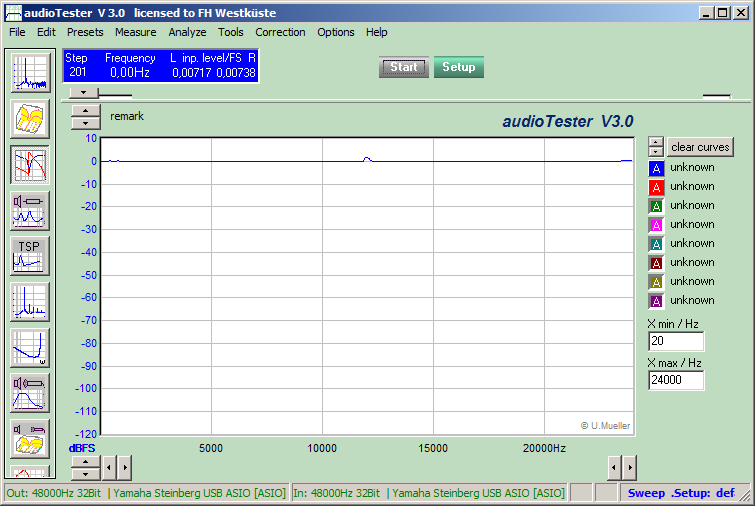
\includegraphics[width=\textwidth]{img/f_gesamt.png}
            \caption{Amplitudengang der gesamten Filterbank}
        \end{figure}
    \end{frame}

    \begin{frame}
        \begin{figure}[p]
            \centering
            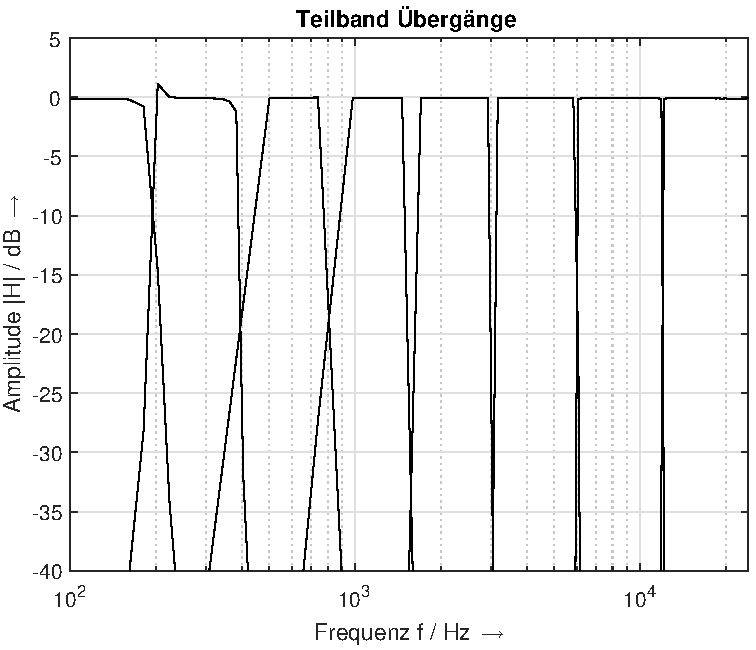
\includegraphics[width=\textwidth]{img/uebergaenge.pdf}
            \caption{�berg�nge zwischen den Teilbandfiltern}
        \end{figure}
    \end{frame}

    \begin{frame}
        \begin{figure}[p]
            \centering
            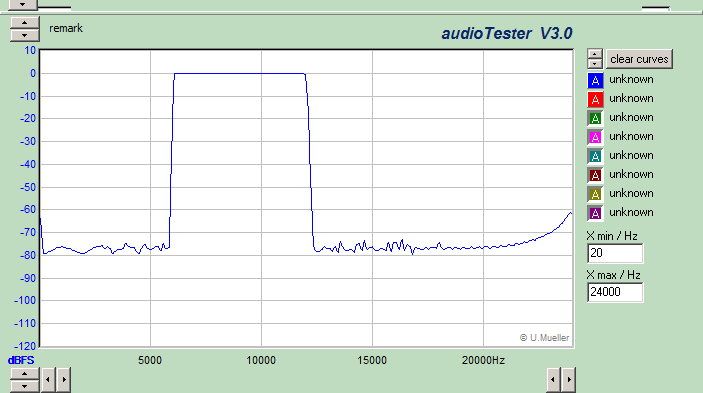
\includegraphics[width=\textwidth]{img/f_hp1.png}
            \caption{Hochpass-Ausgang des 2. Teilbandfilters}
        \end{figure}
    \end{frame}

    \begin{frame}
        \begin{figure}[p]
            \centering
            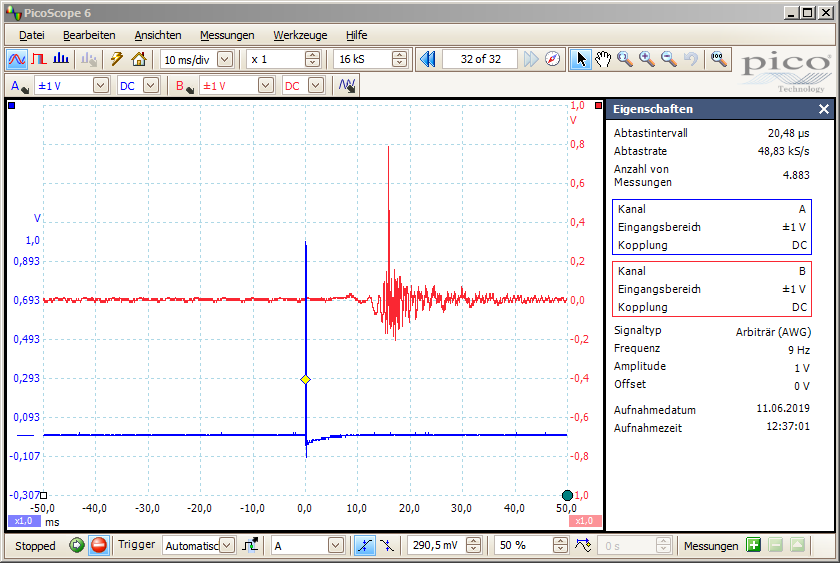
\includegraphics[width=\textwidth]{img/h_gesamt.png}
            \caption{Impulsantwort der Filterbank im Zeitbereich}
        \end{figure}
    \end{frame}


\section{Fazit}

\begin{frame}[allowframebreaks]
  \frametitle{Literatur- und Quellenverzeichnis}
  \bibliographystyle{plainnat}
  \bibliography{literature}
\end{frame}

% ------------------------------------------------
% ----------------------------------------------------------------------------------------

\end{document}
%%% Local Variables:
%%% mode: latex
%%% TeX-master: t
%%% End:
